\documentclass[oneside,final,12pt]{extreport}
\usepackage[utf8]{inputenc} % Исходная строка: \usepackage[koi8-r]{inputenc}
\usepackage[russianb]{babel}
\usepackage{graphicx}
\usepackage{vmargin}
\setpapersize{A4}
\setmarginsrb{2.5cm}{2cm}{1cm}{2cm}{0pt}{0mm}{0pt}{13mm} % Поля по часовой стрелке начиная с "лево"
\usepackage{indentfirst}
\usepackage{cmap} % для кодировки шрифтов в pdf
\linespread{1.3} % полуторный интервал
\renewcommand{\rmdefault}{ftm} % Times New Roman
\sloppy
\begin{document}

\begin{titlepage}
\begin{centering}

Пермский филиал федерального государственного автономного\\
образовательного учреждения высшего образования\\
“Национальный исследовательский университет\\
“Высшая школа экономики”
\vskip2cm
\bf Новый текст\\
\rule{15cm}{1mm}
\vfill
Пермь, 2018

\end{centering}
\end{titlepage}
\setcounter{page}{2}

\tableofcontents
\chapter{Анализ}
\section{Введение}
\par Современное общество невозможно представить без компьютеров. Будь то обычная сим-карта
или дата-центр в несколько десятков гектар площадью, смартфоны, настольные решения,
планшеты, игровые автоматы, сложные системы управления технологическими линиями — всё
это представляет собой компьютер в том или ином виде. Компьютеризация несомненно
затронула все сферы жизнедеятельности человечества. Вычислительные машины являются мощным
инструментом, который упрощает нашу жизнь. Компьютеру не нужен отдых, а вышедшие из строя
детали легко заменить. В последние годы складывается тенденция к развитию слабой форме
искусственного интеллекта — когда компьютер начинает делать выводы по решаемой задаче
самостоятельно, что уже применяется в области медицины и астрономии.
\par Среди массового потребителя очень популярно решение в виде стационарного домашнего
компьютера, который позволяет выполнять игровые и мультимедийные функции. Чаще всего
представляет собой совокупность нескольких компонентов: системный блок, монитор, манипуляторы
ввода (клавиатура, мышь), колонки. Подобная конфигурация позволяет легко заменить любой из
компонентов самостоятельно, не обладая специфичными знаниями или инструментом. Компоненты
системного блока так же представляют из себя отдельные аппаратные решения, которые можно
заменить. Если выбор периферийных устройств не представляет сложную задачу, то выбор
компонентов системного блока — задача требующего особых знаний.
\par Цель данной работы: разработать информационную систему сравнения компьютеров. Основная
задача, которая будет решаться: предоставить техническому специалисту средство, которое
позволит сравнивать конфигурации компьютеров на основании объективной оценки.
\par Тестирую ссылки на изображения. См. рис. \ref{img:01:3dm2}. См. рис. \ref{img:01:002-AIDA64_scr}
\begin{figure}[hp]
	\centering
	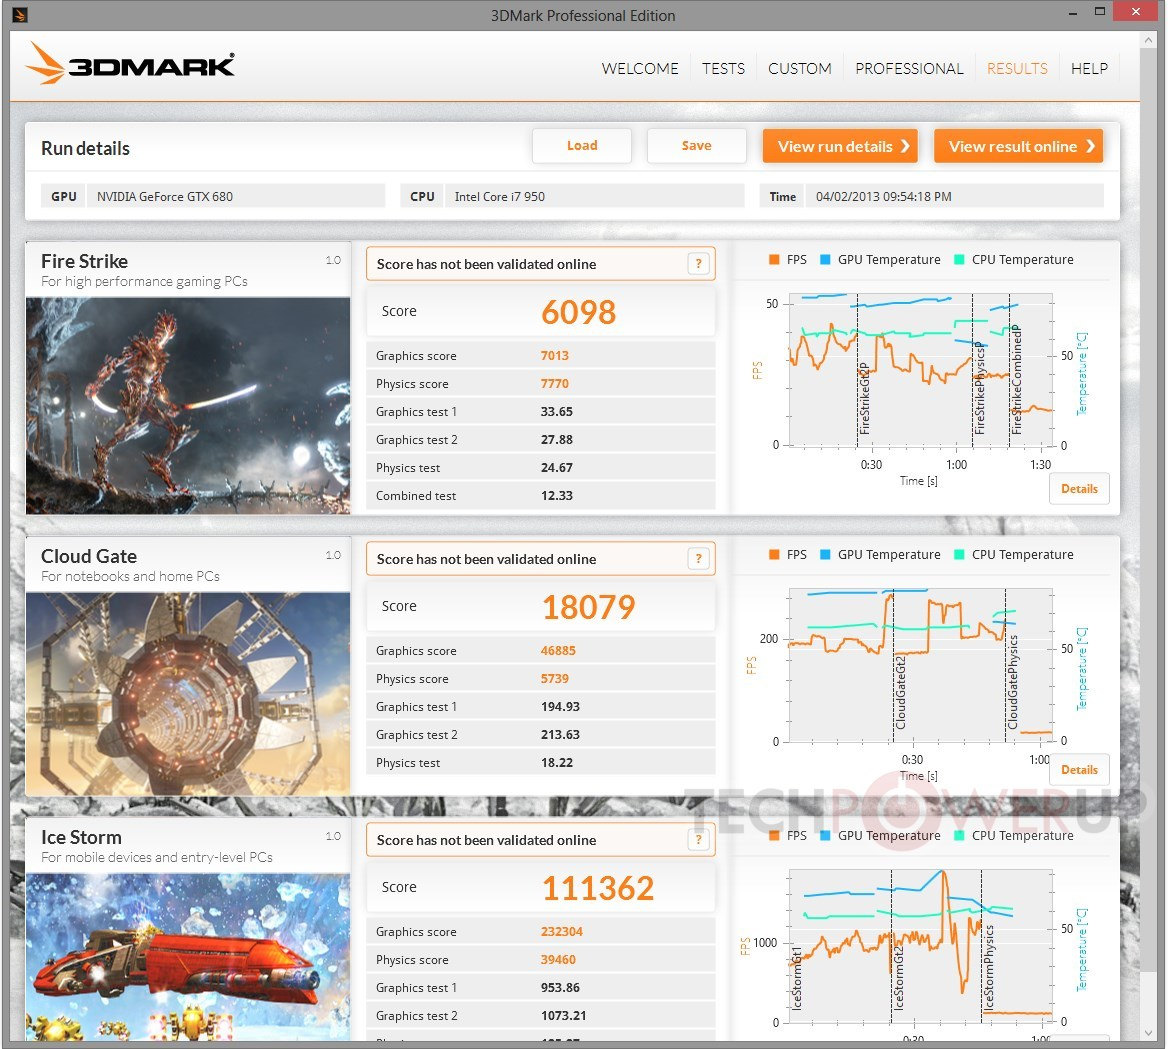
\includegraphics[width=0.7\textwidth]{images/001-3dm2}
	\caption{Подпись рисунка 01}
	\label{img:01:3dm2}
\end{figure}
\begin{figure}[hp]
	\centering
	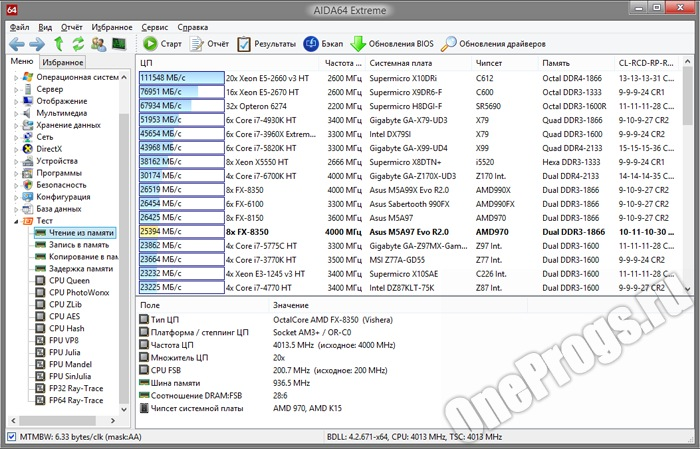
\includegraphics[width=0.7\textwidth]{images/002-AIDA64_scr}
	\caption{Подпись рисунка 02}
	\label{img:01:002-AIDA64_scr}
\end{figure}
\section{Это будет подпункт}
и здесь может быть ваша реклама
\appendix
\chapter{Исходный код}
\section{Модуль filters.py}
Немножечко кода

\begin{verbatim}

from . import models
import django_filters


class DRYFilter(django_filters.FilterSet):
    name = django_filters.CharFilter(lookup_expr='icontains')
    score = django_filters.RangeFilter()
    rank = django_filters.NumberFilter()
    in_stock = django_filters.BooleanFilter()
    price = django_filters.RangeFilter()

\end{verbatim}

\end{document}